\documentclass[journal = jacsat, manuscript = article, layout = twocolumn]{achemso}

\usepackage[version = 4]{mhchem}
\usepackage{graphicx}
\usepackage{mwe}
\usepackage[labelfont=bf]{caption}

% disable symbol next to email
\makeatletter
\def\acs@author@fnsymbol#1{}
\makeatother
% enable abstract
\AbstractOn
% put abstract and title on the same page
\let\oldmaketitle\maketitle
\let\maketitle\relax
% shut up latex
\hbadness=99999

% macros
\newcommand{\nidppe}{\ce{Ni(dppe)Cl2}}
\newcommand{\nicl}{\ce{NiCl2 $\cdot$ 6H2O}}
\newcommand{\nh}{\ce{NH3}}
\newcommand{\nanh}{\ce{Na $\cdot$ NH3}}
\newcommand{\nhbr}{\ce{NH4Br}}
\newcommand{\h}{$^1$H}
\newcommand{\p}{$^{31}$P}
\newcommand{\cdcl}{\ce{CDCl3}}
\newcommand{\niion}{\ce{Ni^{2+}}}
\newcommand{\wavenum}{cm$^{-1}$}
\newcommand{\del}[1]{$\delta=#1$}

\title{1,2-bis(diphenylphosphino)ethane (dppe) and \nidppe\ synthesis via
solvated electron reduction}

\author{David Qiu}
\affiliation{Department of Chemistry, University of Illinois at
Urbana-Champaign, 505 S Matthews Avenue, Urbana, IL, 61801}
\email{davidlq2@illinois.edu}

\begin{document}

%%%%%%%%%%%%%%%%%%%%%%%%%%%%%%%%%%%%%%%%%%%%%%%%%%%%%%%%%%%%%%%%%%%%%%%%%%%%%%%%
% Abstract
%%%%%%%%%%%%%%%%%%%%%%%%%%%%%%%%%%%%%%%%%%%%%%%%%%%%%%%%%%%%%%%%%%%%%%%%%%%%%%%%

\twocolumn[
\begin{@twocolumnfalse}
\oldmaketitle
\hrule
\begin{abstract}

This experiment demonstrated successful synthesis of the dppe ligand via
solvated electron reduction of triphenylphosphine followed by treatment with
1,2-dichloroethane. Subsequent ligand substitution of \nicl\ yielded \nidppe.
The reaction had an overall yield of 118\% for dppe and 47\% for \nidppe. \h\
NMR, \p\ NMR, and IR spectra of dppe and \nidppe\ were analyzed, and confirmed
experimental success while noting the presence of excess solvent and residual
impurity. Future studies should improve upon this synthesis by minimizing
residual solvent via vacuum, improving \nidppe\ yield via temperature control,
and using higher resolution NMR instruments to characterize dppe.

\end{abstract}
\hrule
\vspace{6mm}%
\end{@twocolumnfalse}
]

%%%%%%%%%%%%%%%%%%%%%%%%%%%%%%%%%%%%%%%%%%%%%%%%%%%%%%%%%%%%%%%%%%%%%%%%%%%%%%%%
% Introduction
%%%%%%%%%%%%%%%%%%%%%%%%%%%%%%%%%%%%%%%%%%%%%%%%%%%%%%%%%%%%%%%%%%%%%%%%%%%%%%%%

Economical synthesis of ligands and metal complexes using readily available
reagents are of vital importance in both laboratory and industry. Polymer
chemistry relies almost entirely on catalysts formed from these reactions. The
Ziegler-Natta metallocene catalysts (e.g.\ \ce{Cp2ZrCl2}), which are still used
today to generate polyethylene, are one famous example. Their efficacy depends
on the metallocene ligands, which occupy multiple coordination sites while being
too sterically hindered to fully chelate the metal ion. This property prevents
excessive termination and other undesirable reactions during polymerization.
\cite{ziegler-natta}

A bulky, polydentate ligand such as dppe shares this property, making dppe
complexes useful polymerization catalysts. This catalytic ability is exhibited
in \nidppe, which is already known to promote chain growth and cross-coupling of
aromatic molecules. \cite{nidppe-intro-1, nidppe-intro-2, dppenmr1}

\begin{figure}[H]
	
\includegraphics[width=0.475\textwidth]{figures/scheme.png}
	\caption*{\textbf{Scheme 1:} Synthesis of dppe via reduction of
	triphenylphosphine followed by reaction with 1,2-dichloroethane.}
\end{figure}

\begin{figure}[H]
	
\includegraphics[width=0.4\textwidth]{figures/scheme-2.png}
	\caption*{\textbf{Scheme 2:} Synthesis of \nidppe\ via direct ligand
	substitution of \nicl.}
\end{figure}

% put NMR spectra on next page
% twocolumn format is dumb; it puts figures on the next page
\begin{figure*}[t]
	\center
	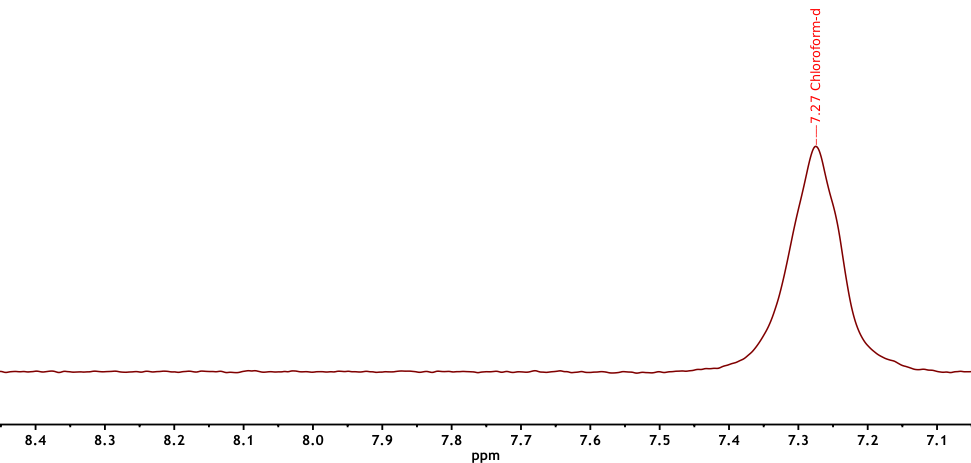
\includegraphics[width=0.7\textwidth]{figures/zoom_dppe_hnmr.png}
	\caption{\h\ NMR of dppe, magnified to highlight the aromatic shifts at
	\del 7.27 ppm. Note the overlap with the existing \cdcl\ peak.}

	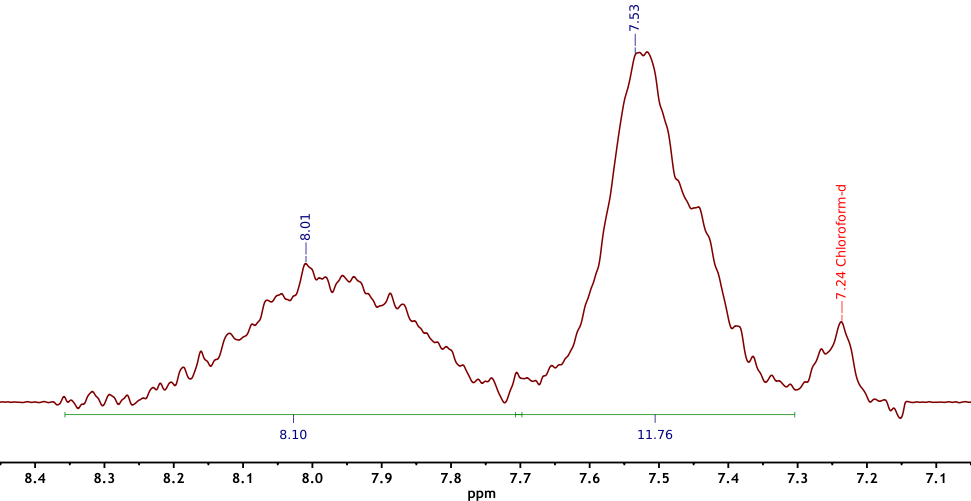
\includegraphics[width=0.7\textwidth]{figures/zoom_nidppe_hnmr.png}
	\caption{\h\ NMR of \nidppe, magnified to highlight the aromatic shifts
	at \del 8.01 ppm (8 H) and \del 7.53 (12 H). Note the distinguished
\cdcl\ peak (\del 7.24 ppm) upon formation of the nickel complex.}
\end{figure*}

This experiment aimed to achieve economical synthesis of both the dppe ligand
and \nidppe\ complex for use in polymer chemistry. The synthetic route thus
needed to maximize usage of readily available reagents for synthesis.
Triphenylphosphine was chosen as a precursor for dppe due to its availability
and structural similarity. Na and \nh, both of which are also readily available,
were chosen to perform solvated electron reduction on triphenylphosphine, which
would yield the dppe ligand upon subsequent reaction with 1,2-dichloroethane
(Scheme 1). The newly-synthesized dppe ligand was then reacted with \nicl\ to
yield the polymerization catalyst \nidppe\ (Scheme 2).

%%%%%%%%%%%%%%%%%%%%%%%%%%%%%%%%%%%%%%%%%%%%%%%%%%%%%%%%%%%%%%%%%%%%%%%%%%%%%%%%
% Results and Discussion
%%%%%%%%%%%%%%%%%%%%%%%%%%%%%%%%%%%%%%%%%%%%%%%%%%%%%%%%%%%%%%%%%%%%%%%%%%%%%%%%

The experiment resulted in a 118\% yield of dppe, and a 47\% yield of
\nidppe. The dppe sample thus contained some residual impurity or solvent,
analysis of which is discussed later. The yield of \nidppe\ is interesting as
well, as it implies that the ligand substitution reaction (Scheme 2) was not
driven to completion. This could be a result of either poor kinetics arising
from reaction conditions (room temperature, short reaction time), or
thermodynamic effects driving the reaction towards dissociation due to steric
effects of the dppe ligand. However, this is unlikely as metal chelates are
known to be highly stable \cite{textbook}. Furthermore, existing literature
support the kinetic hypothesis, as yields above 90\% were achieved at higher
temperatures in 2-propanol. \cite{dppenmr1}

To further investigate these findings, the 60 MHz \h\ and 400 MHz \p\ NMR
spectra in \cdcl\ were taken and analyzed. The \h\ NMR spectrum of dppe was
rather poor; ethanol was a prominent impurity, and shifts corresponding to the
aromatic hydrogens were not discernible in the \h\ NMR spectra (Figure 1). These
are due both to the poor resolution of the 60 MHz instrument and overlap with
the \cdcl\ solvent peak.

This finding has been replicated in the literature \cite{dppenmr1}, and is
further evidenced by the \h\ NMR spectrum of \nidppe\ (Figure 2), which had
distinguishable aromatic shifts unlike the \h\ NMR spectrum of dppe (c.f.\
Figure 1). This is because the presence of the \niion\ metal center withdraws
electron density from the lone pairs of phosphorus and the aromatic protons,
causing them to appear further downfield and distinguishing the protons meta to
phosphorus from those that are ortho or para to phosphorus.  This rationale is
supported by the integration underneath each aromatic peak in Figure 2, which
distinguishes the 8 meta protons to the 12 ortho and para protons.

The \p\ NMR spectra were not particularly revealing, as there exists only one
chemically distinct phosphorus nucleus in both dppe and \nidppe. However, there was
either an unknown impurity or an instrumental artifact at \del -105.91 ppm and
\del -221.00 ppm observed in both \p\ NMR spectra of dppe and \nidppe. This
finding was not replicated elsewhere, suggesting that its corresponding
impurities are unique to this synthetic method, or that the artifacts are unique
to the NMR instrument used in this experiment.

Aside from the aforementioned impurities, artifacts, and \h\ NMR multiplicities
(indistinguishable due to the poor resolution), the \h\ and \p\ spectra are in
good agreement with existing NMR studies done on dppe and \nidppe.
\cite{dppenmr1, dppenmr2}

The IR spectrum of dppe was not noteworthy, and indicated exclusively a C-H
stretch, an aromatic C--C/C=C stretch, and an O-H stretch corresponding to
ethanol. Interestingly, the IR spectrum of \nidppe\ was completely absent in the
3000--4000 \wavenum\ region, and exhibited purely an aromatic C--C/C=C stretch.
This is largely consistent with existing IR spectra of \nidppe\ in
literature\cite{dppeir}, which indicate exceedingly weak C-H stretches in
\nidppe.

In conclusion, this experiment demonstrated the successful synthesis of the dppe
ligand via solvated electron reduction of triphenylphosphine followed by
treatment with 1,2-dichloroethane, as well as subsequent ligand substitution to
yield \nidppe. As indicated by the \h\ NMR, \p\ NMR, and IR analysis, future
studies should improve upon this synthesis by minimizing residual solvent (e.g.
by drying the sample under vacuum prior to analysis), improving \nidppe\
yield via temperature control, and using higher resolution NMR instruments to
characterize dppe.

\bibliography{lab_3.bib}

\end{document}
